\chapter{Motivación}
\section{Introducción}
Los conceptos de motivación se utilizan para modelar las motivaciones, o razones, que subyacen en el diseño o cambio de alguna arquitectura empresarial. Estas motivaciones influyen, orientan y limitan el diseño.
\paragraph{}
Es esencial comprender los factores, a menudo referidos como conductores, que influyen en los elementos motivacionales. Pueden originarse desde dentro o fuera de la empresa. Los conductores internos, también llamados preocupaciones, están asociados con las partes interesadas, que pueden ser algún ser humano individual o algún grupo de seres humanos, como un equipo de proyecto, empresa o sociedad. rentabilidad. Es común que las empresas realicen una evaluación de estos conductores; Por ejemplo, utilizando un análisis DAFO, con el fin de responder de la mejor manera.
\paragraph{}
Las motivaciones reales están representadas por objetivos, principios, requisitos y limitaciones. Los objetivos representan algún resultado deseado - o final - que un interesado quiere lograr; Por ejemplo, aumentando la satisfacción del cliente en un 10. Los principios y los requisitos representan las propiedades deseadas de las soluciones - o medios - para realizar las metas. Los principios son pautas normativas que guían el diseño de todas las soluciones posibles en un contexto dado. Por ejemplo, el principio "Los datos deben almacenarse sólo una vez" representa un medio para lograr el objetivo de "consistencia de datos" y se aplica a todos los posibles diseños de la arquitectura de la organización. Los requisitos representan declaraciones formales de necesidad, expresadas por los interesados, que deben ser satisfechas por la arquitectura o las soluciones. Por ejemplo, el requisito "Usar un único sistema de CRM" se ajusta al principio antes mencionado aplicándolo a la arquitectura de la organización actual en el contexto de la gestión de los datos de los clientes.
\newpage
\section{Punto de Vista de Stakeholder}

\subsection{Modelo}
\begin{figure}[th!]
	\centering
	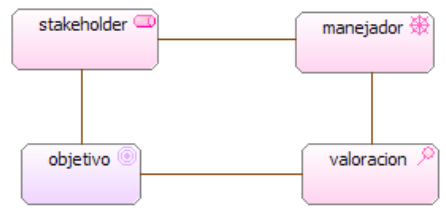
\includegraphics[width=0.7\linewidth]{arquitectura/imagenes/modeloStakeholder}
	\caption{Metamodelo Punto de Vista de Partes Interesadas}
	\label{metamodelo partes interesadas}
\end{figure}
El punto de vista de las partes interesadas permite al analista modelar las partes interesadas, los impulsores internos y externos del cambio y las evaluaciones (en términos de fortalezas, debilidades, oportunidades y amenazas) de estos controladores. También se pueden describir los vínculos con los objetivos iniciales (de nivel alto) que abordan estas preocupaciones y evaluaciones. Estos objetivos forman la base para el proceso de ingeniería de requisitos, incluyendo refinamiento de objetivos, contribución y análisis de conflictos, y la derivación de requisitos que realicen los objetivos


\subsection{Caso  de estudio}

\begin{figure}[th!]
	\centering
	\includegraphics[width=0.6\linewidth]{arquitectura/imagenes/PuntoVistaStakeholder}
	\caption{Modelo Punto de Vista de Partes Interesadas}
	\label{modelopartesinteresadas}
\end{figure}

En  este punto de vista de la figura \ref{modelopartesinteresadas} se puede observar como las dos partes interesadas son la tienda JSJSports y se relacionan por medio del objetivo de vender artículos deportivos, puesto que a JSJSport le interesa vender productos y a el cliente comprarlos, este objetivo se mide por medio del reconocimiento que adquiere JSJSports nacional e internacional mente.\newline
Ademas del objetivo de la venta el cliente tiene el objetivo de conseguir productos de calidad conforme a sus deseos específicos, este objetivo se mide si se logra que el cliente consiga el producto que desea en la tienda y de la mejor calidad.


\newpage

\section{Punto de Vista de Realización de Objetivos}

\subsection{Modelo}

\begin{figure}[th!]
	\centering
	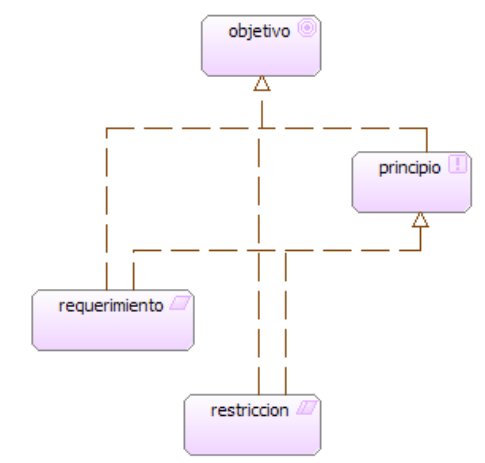
\includegraphics[width=0.4\linewidth]{arquitectura/imagenes/modeloRealizacionObjetivos}
	\caption{Metamodelo Punto de Vista de Realización de Objetivos}
	\label{metamodelo realizacion objetivos}
\end{figure}
El punto de vista de la realización de metas permite a un diseñador modelar el refinamiento de metas (de alto nivel) en metas más concretas y el refinamiento de objetivos concretos en requisitos o restricciones que describen las propiedades que se necesitan para realizar las metas. El refinamiento de objetivos en subobjetivos se modela utilizando la relación de agregación. El refinamiento de metas en requisitos se modela utilizando la relación de realización.
Además, los principios pueden ser modelados que guían el refinamiento de objetivos en requisitos

\subsection{Caso de Estudio}

\begin{figure}[th!]
	\centering
	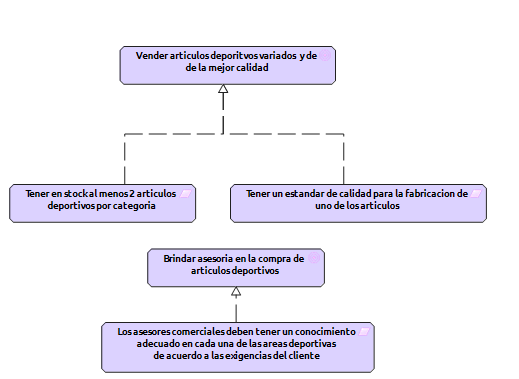
\includegraphics[width=0.5\linewidth]{arquitectura/imagenes/PuntoVistaRealizacionObjetivos}
	\caption{Modelo Punto de Vista de Realización de Objetivos}
	\label{ModeloRealizacionObjetivos}
\end{figure}

En la figura \ref{ModeloRealizacionObjetivos} se pueden los dos objetivos principales de la empresa JSJSPorts, el primero de estos es el de vender artículos deportivos de la mejor calidad y de todo tipo, este tiene dos requerimientos, estos son el de tener en stock por lo menos 2 artículos diferentes para cada disciplina deportiva y el de tener un estandar que defina la calidad de estos productos.\newline
El segundo objetivo  es el de brindar asesoría al cliente en el proceso de compra al cliente, el cumplimiento de  este objetivo requiere que los asesores tengan un conocimiento sobre cada una de las disciplinas y los artículos que se pueden recomendar al cliente según sus requerimientos.

\newpage

\section{Punto de Vista de contribución de Objetivos}

\subsection{Modelo}
\begin{figure}[th!]
	\centering
	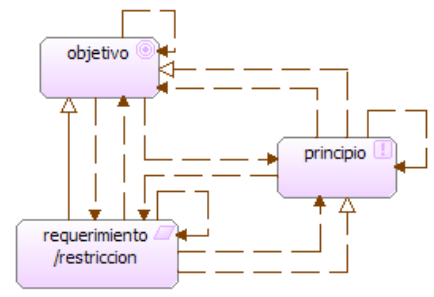
\includegraphics[width=0.6\linewidth]{arquitectura/imagenes/modeloContribucion}
	\caption{Metamodelo Punto de Vista de Contribucion}
	\label{metamodelo contribucion}
\end{figure}
El punto de vista de la contribución permite a un diseñador o analista modelar las relaciones de influencia entre objetivos y requisitos. Las vistas resultantes pueden usarse para analizar el impacto que las metas tienen entre sí o para detectar conflictos entre los objetivos de las partes interesadas.
Típicamente, este punto de vista puede ser utilizado después de que los objetivos se hayan refinado hasta cierto punto en subobjetivos y, posiblemente, en requisitos.

\subsection{Caso de Estudio}

\begin{figure}[th!]
	\centering
	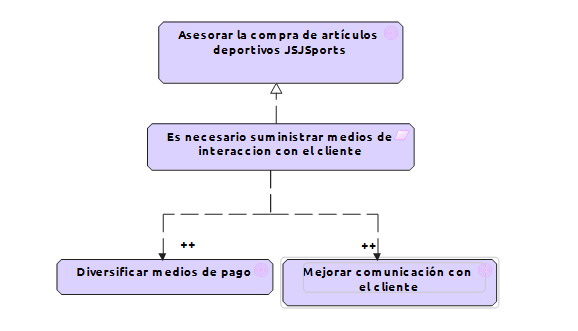
\includegraphics[width=0.9\linewidth]{arquitectura/imagenes/PuntoVistaContribucion}
	\caption{Modelo Punto de Vista de Contribucion}
	\label{modelocontribucion}
\end{figure}

En el modelo de contribución en la figura \ref{modelocontribucion} se puede observar como para garantizar el cumplimiento del objetivo de asesorar la compra de artículos deportivos es necesario garantizar medios suficientes de interacción con el cliente, esto se logra Diversificando los medios de pago y mejorando la comunicación con los clientes.

\newpage

\section{Punto de Vista de Principios}

\subsection{Modelo}

\begin{figure}[th!]
	\centering
	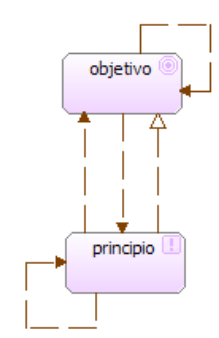
\includegraphics[width=0.3\linewidth]{arquitectura/imagenes/modeloPrincipios}
	\caption{Metamodelo Punto de Vista de Principios}
	\label{metamodelo principios}
\end{figure}
El punto de vista de los principios permite al analista o diseñador modelar los principios que son relevantes para el problema de diseño en cuestión, incluyendo los objetivos que motivan estos principios. Además, las relaciones entre los principios y sus objetivos pueden ser modeladas. 

\subsection{Caso de Estudio}
\begin{figure}[th!]
	\centering
	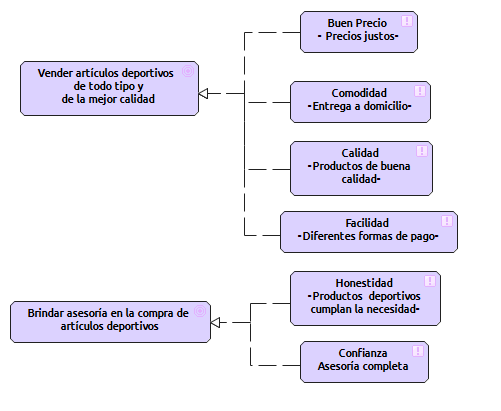
\includegraphics[width=0.4\linewidth]{arquitectura/imagenes/PuntoVistaPrincipios}
	\caption{Modelo Punto de Vista de Principios}
	\label{modelo principios}
\end{figure}

En la figura \ref{modelo principios} se puede observar los dos objetivos principales del problema y los objetivos que motivan estos principios, en este caso al objetivo de vender artículos deportivos vemos que lo soportan los principios de un buen precio que sea justo para el cliente y la tienda, la comodidad de recibir el producto en su ubicación, el principio de la mejor calidad en cada uno de los productos que se ofrecen
 y como último la facilidad que se le brinda al cliente de pagar de diferentes formas.\newline
El objetivo de brindar asesoría al cliente se basa en los principios de honestidad y confianza que puede tener el cliente de que su proceso de compra sera totalmente claro y lo que se le recomienda es lo que le conviene.
\newpage

\section{Punto de Vista de Realización de Requerimientos}

\subsection{Modelo}

\begin{figure}[th!]
	\centering
	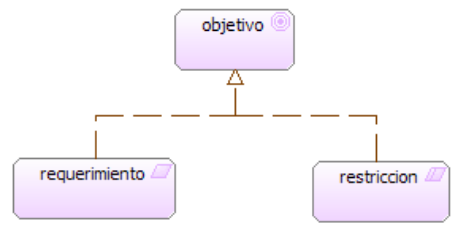
\includegraphics[width=0.7\linewidth]{arquitectura/imagenes/modeloRealizacionRequerimientos}
	\caption{Metamodelo Punto de Vista de Realización de Requerimientos}
	\label{metamodelo realizacion requerimientos}
\end{figure}
El punto de vista de la realización de los requisitos permite al diseñador modelar la realización de los requisitos por parte de los elementos básicos, como los actores empresariales, los servicios empresariales, los procesos empresariales, los servicios de aplicación, los componentes de la aplicación, etc.
Además, este punto de vista puede usarse para refinar requisitos en requisitos más detallados. La relación de agregación se utiliza para este propósito.

\subsection{Caso de Estudio}

\begin{figure}[th!]
	\centering
	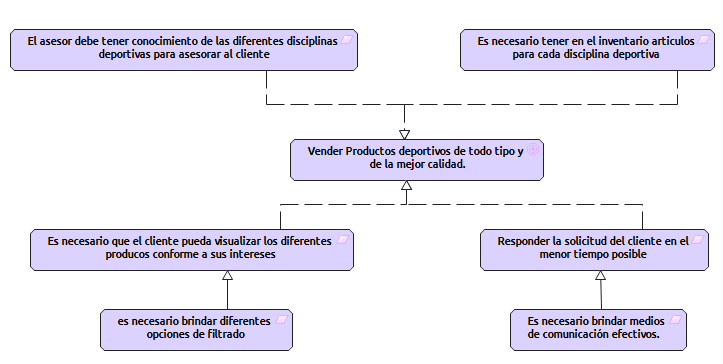
\includegraphics[width=0.7\linewidth]{arquitectura/imagenes/PuntoVistaRealizacionRequerimientos}
	\caption{Modelo Punto de Vista de Realización de Requerimientos}
	\label{modelo realizacion requerimientos}
\end{figure}

En este punto de vista se puede observar cada uno de los requerimientos que soportan el objetivo de vender artículos deportivos de todo tipo para cada disciplina deportiva y de la mejor calidad, en la figura \ref{modelo realizacion requerimientos} se pueden observar 4 requerimientos principales, el primero se refiera a que el asesor debe contar con los conocimientos necesarios para poder brindar una correcta asesoría al cliente, el segundo busca garantizar que el cliente encuentre lo que busca en la tienda virtual, el tercero se refiere a la forma en el que el cliente puede buscar los productos y la forma en que este selecciona lo que le interesa para este es necesario que garantizar diferentes tipos de filtros y el último de los requerimientos se refiere a la velocidad con que un asesor responde la solicitud de un cliente, de este requerimiento se extiende el requerimiento de contar con un buen medio de comunicación.
\newpage

\section{Punto de Vista de Motivación}

\subsection{Modelo}
\begin{figure}[th!]
	\centering
	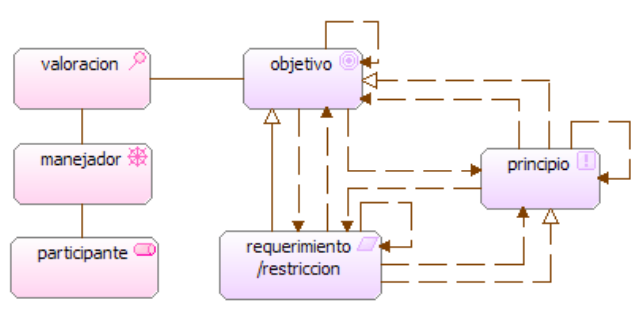
\includegraphics[width=0.7\linewidth]{arquitectura/imagenes/modeloMotivacion}
	\caption{Metamodelo Punto de Vista de Motivación}
	\label{metamodelo motivacion}
\end{figure}
El punto de vista de la motivación permite al diseñador o analista modelar el aspecto de la motivación, sin centrarse en ciertos elementos dentro de este aspecto. Por ejemplo, este punto de vista puede utilizarse para presentar un panorama completo o parcial del aspecto de la motivación relacionando a las partes interesadas, sus objetivos principales, los principios que se aplican y los principales requisitos de servicios, procesos, aplicaciones y objetos.

\subsection{Caso de estudio}

\begin{figure}[th!]
	\centering
	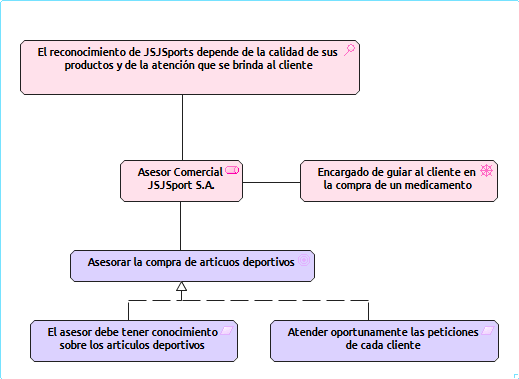
\includegraphics[width=0.7\linewidth]{arquitectura/imagenes/PuntoVistaMotivacion}
	\caption{Modelo Punto de Vista de Motivación}
	\label{modelo motivacion}
\end{figure}


En este punto de vista se puede observar un panorama de todo el aspecto de motivación del proyecto en este caso se ve al stakeholder Asesor Comercial, con su valoración y su manejador respectivo, además de esto se ve el objetivo principal con el que este cumple y los requerimientos que lo soportan en este caso, para el asesor, los requerimientos son conocer los artículos deportivos y las disciplinas para las que estos se ofertan y el de atender oportunamente las peticiones de cada cliente.

\newpage

